%\documentclass[AER]{AEA}
\documentclass[12pt]{report}
%\documentclass[12pt]{article}
%\documentclass[12pt,a4paper]{article}

\usepackage[utf8]{inputenc}


\usepackage{mathtools}
\usepackage{amsmath}
\usepackage{amssymb}
\usepackage{amsthm}

\usepackage{float}
%\usepackage[cmbold]{mathtime}
%\usepackage{mt11p}
\usepackage{placeins}
\usepackage{caption}
\usepackage{color}
\usepackage{subfigure}
\usepackage{multirow}
\usepackage{epsfig}
\usepackage{listings}
\usepackage{enumitem}
\usepackage{rotating,tabularx}
%\usepackage[graphicx]{realboxes}
\usepackage{graphicx}
\usepackage{graphics}
\usepackage{epstopdf}
\usepackage{longtable}
\usepackage[pdftex]{hyperref}
%\usepackage{breakurl}
\usepackage{epigraph}
\usepackage{xspace}
\usepackage{amsfonts}
\usepackage{eurosym}
\usepackage{ulem}

\usepackage{tikz}
\usetikzlibrary{spy}

\usepackage{verbatim}



\usepackage{footmisc}
\usepackage{comment}
\usepackage{setspace}
\usepackage{geometry}
\usepackage{caption}
\usepackage{pdflscape}
\usepackage{array}
\usepackage[authoryear]{natbib}
\usepackage{booktabs}
\usepackage{dcolumn}
\usepackage{mathrsfs}
%\usepackage[justification=centering]{caption}
%\captionsetup[table]{format=plain,labelformat=simple,labelsep=period,singlelinecheck=true}%
\bibliographystyle{apalike}
%\bibliographystyle{unsrtnat}



%\bibliographystyle{aea}
\usepackage{enumitem}
\usepackage{tikz}
\usetikzlibrary{positioning}
\usetikzlibrary{arrows}
\usetikzlibrary{shapes.multipart}

\usetikzlibrary{shapes}
\def\checkmark{\tikz\fill[scale=0.4](0,.35) -- (.25,0) -- (1,.7) -- (.25,.15) -- cycle;}
%\usepackage{tikz}
%\usetikzlibrary{snakes}
%\usetikzlibrary{patterns}

%\draftSpacing{1.5}

\usepackage{xcolor}
\hypersetup{
colorlinks,
linkcolor={blue!50!black},
citecolor={blue!50!black},
urlcolor={blue!50!black}}

%\renewcommand{\familydefault}{\sfdefault}
%\usepackage{helvet}
%\setlength{\parindent}{0.4cm}
%\setlength{\parindent}{2em}
%\setlength{\parskip}{1em}

%\normalem

%\doublespacing
\onehalfspacing
%\singlespacing
%\linespread{1.5}

\newtheorem{theorem}{Theorem}
\newtheorem{corollary}[theorem]{Corollary}
\newtheorem{proposition}{Proposition}
\newtheorem{definition}{Definition}
\newtheorem{axiom}{Axiom}
\newtheorem{observation}{Observation}
\newtheorem{assumption}{Assumption}	
\newtheorem{remark}{Remark}
\newtheorem{lemma}{Lemma}
\newtheorem{result}{result}


\newcommand{\ra}[1]{\renewcommand{\arraystretch}{#1}}

\newcommand{\E}{\mathrm{E}}
\newcommand{\Var}{\mathrm{Var}}
\newcommand{\Corr}{\mathrm{Corr}}
\newcommand{\Cov}{\mathrm{Cov}}

\newcolumntype{d}[1]{D{.}{.}{#1}} % "decimal" column type
\renewcommand{\ast}{{}^{\textstyle *}} % for raised "asterisks"

\newtheorem{hyp}{Hypothesis}
\newtheorem{subhyp}{Hypothesis}[hyp]
\renewcommand{\thesubhyp}{\thehyp\alph{subhyp}}

\newcommand{\red}[1]{{\color{red} #1}}
\newcommand{\blue}[1]{{\color{blue} #1}}

%\newcommand*{\qed}{\hfill\ensuremath{\blacksquare}}%

\newcolumntype{L}[1]{>{\raggedright\let\newline\\arraybackslash\hspace{0pt}}m{#1}}
\newcolumntype{C}[1]{>{\centering\let\newline\\arraybackslash\hspace{0pt}}m{#1}}
\newcolumntype{R}[1]{>{\raggedleft\let\newline\\arraybackslash\hspace{0pt}}m{#1}}

%\geometry{left=1.5in,right=1.5in,top=1.5in,bottom=1.5in}
\geometry{left=1in,right=1in,top=1in,bottom=1in}

\epstopdfsetup{outdir=./}

\newcommand{\elabel}[1]{\label{eq:#1}}
\newcommand{\eref}[1]{Eq.~(\ref{eq:#1})}
\newcommand{\ceref}[2]{(\ref{eq:#1}#2)}
\newcommand{\Eref}[1]{Equation~(\ref{eq:#1})}
\newcommand{\erefs}[2]{Eqs.~(\ref{eq:#1}--\ref{eq:#2})}

\newcommand{\Sref}[1]{Section~\ref{sec:#1}}
\newcommand{\sref}[1]{Sec.~\ref{sec:#1}}

\newcommand{\Pref}[1]{Proposition~\ref{prop:#1}}
\newcommand{\pref}[1]{Prop.~\ref{prop:#1}}
\newcommand{\preflong}[1]{proposition~\ref{prop:#1}}

\newcommand{\Aref}[1]{Axiom~\ref{ax:#1}}

\newcommand{\clabel}[1]{\label{coro:#1}}
\newcommand{\Cref}[1]{Corollary~\ref{coro:#1}}
\newcommand{\cref}[1]{Cor.~\ref{coro:#1}}
\newcommand{\creflong}[1]{corollary~\ref{coro:#1}}

\newcommand{\etal}{{\it et~al.}\xspace}
\newcommand{\ie}{{\it i.e.}\ }
\newcommand{\eg}{{\it e.g.}\ }
\newcommand{\etc}{{\it etc.}\ }
\newcommand{\cf}{{\it c.f.}\ }
\newcommand{\ave}[1]{\left\langle#1 \right\rangle}
\newcommand{\person}[1]{{\it \sc #1}}

\newcommand{\AAA}[1]{\red{{\it AA: #1 AA}}}
\newcommand{\YB}[1]{\blue{{\it YB: #1 YB}}}

\newcommand{\flabel}[1]{\label{fig:#1}}
\newcommand{\fref}[1]{Fig.~\ref{fig:#1}}
\newcommand{\Fref}[1]{Figure~\ref{fig:#1}}

\newcommand{\tlabel}[1]{\label{tab:#1}}
\newcommand{\tref}[1]{Tab.~\ref{tab:#1}}
\newcommand{\Tref}[1]{Table~\ref{tab:#1}}

\newcommand{\be}{\begin{equation}}
\newcommand{\ee}{\end{equation}}
\newcommand{\bea}{\begin{eqnarray}}
\newcommand{\eea}{\end{eqnarray}}

\newcommand{\bi}{\begin{itemize}}
\newcommand{\ei}{\end{itemize}}

\newcommand{\Dt}{\Delta t}
\newcommand{\Dx}{\Delta x}
\newcommand{\Epsilon}{\mathcal{E}}
\newcommand{\etau}{\tau^\text{eqm}}
\newcommand{\wtau}{\widetilde{\tau}}
\newcommand{\xN}{\ave{x}_N}
\newcommand{\Sdata}{S^{\text{data}}}
\newcommand{\Smodel}{S^{\text{model}}}

\newcommand{\del}{D}
\newcommand{\hor}{H}



\setlength{\parindent}{0.0cm}
\setlength{\parskip}{0.4em}

\numberwithin{equation}{section}
\DeclareMathOperator\erf{erf}


\begin{document}

\title{Monopoly, Piracy and network value}
\author{Diomides Mavroyiannis}

\maketitle

\begin{abstract}
This paper presents a model for the consumption of a \textit{cultural} good where consumers can either purchase or pirate the good (or not consume it). Because of the specificity of the \textit{cultural} good, active consumers (users), buyers and pirates, derive a network utility that depends on the numbers of users of the goods with which they can share their experience of the cultural good. It is shown that the monopoly firm selling the cultural good may obtain a higher profit when piracy is possible than when it is not. Consequently, it is presented that increasing the cost of piracy has a non monotonic effect on a firm's profit and welfare.
\end{abstract}

\noindent\textbf{Keywords: Monopoly, Piracy, Network goods, Industrial Organization}

\section{Introduction}

The music industry is often seen as the primary victim of piracy. It's long term reduction in profit has been attributed to the large number of pirates whose actions allegedly harm both artists and their representatives\citep{B03}. Still, more recent analysis estimates that as many copies of popular music are being pirated as are being accessed through legal means (\citep{O15}).

\iffalse
Piracy is the term used throughout this paper to describe the copying of a digital good without the permission of the one who owns the intellectual property in question. Since in essence this digital good is an idea, the supply of it is infinite. If for instance somebody pirates a song and plays it, what she really pirated is the specific sequence of frequencies that her speakers are emitting. Fundamentally this is equivalent to a carpenter observing another carpenter construct something and then mimicking the process with his own materials. Piracy is in essence the restructuring of ones  own property without the permission of the person who has originally re-structured his property in that way.

What makes digital piracy different from merely copying? Whilst copying inherently has a noise to it which makes the copy imperfect, piracy is often considered as a perfect copy. Here we can already perhaps describe why piracy may be less desirable than copying. The process of copying itself may be innovative as an imperfect copy will sometimes create a spin-off which is superior to the original, so the process of copying in itself may be welfare improving. Attempts at approximations may yield outcomes that are superior to the original, this is especially true if there is noise in more than one dimension.

On the other hand the concept of a perfect copy is often too quickly employed, most purchased goods do not come merely with just an instance of the product but come with a bundle of goods or promise of future services. It is unclear if we can truly call a pirated version of a song and legally downloaded equivalent an identical product because the process of acquisition itself may not be neutral. Things such as accessibility and user interface also undoubtedly play a role.
\fi

The magnitude of the damage caused by piracy is ambiguous. Given the fact that some artists choose to give their work away for free, it may be inferred that piracy does not always harm the actors of the sector. Music is often uploaded for free on public platforms or even freely uploaded on piracy sites by their creators. The potential rise of the revenue of complementary goods such as concerts may compensate the direct loss on the sale of music. However, it remains unclear to which extent this entirely compensates for the loss in direct music sales. There also exist large movements against piracy. Many industry experts and artists argue that it is not possible to maintain a high level of innovation in the sector without protecting the market from pirates.

The main examples of digital goods which have a piracy option are music, movies or televised series. The main alternative to buying usually takes the form of torrents or online streaming. Buying on the other hand may take the form of renting or purchasing a copy of the product. For instance Spotify, the music platform, is essentially a streaming service which also allows users to download songs.

For the \textit{cultural} goods that we consider, the users' utility depends mainly on two components:  intrinsic valuation and extrinsic valuation of the good. The intrinsic valuation of the good is the utility that the user derives when he consumes the good independently of the actions of other consumers. The extrinsic valuation is the utility that the user derives when he consumes the good which depends on others consumers' choices. With the second element, we intend to represent the fact that the value of a cultural good also depends on the possibility to exchange about it with members of your social network and the higher the possible exchanges are, the more consumption of the cultural is enjoyed. 


There exist many types of goods which have large extrinsic portion to their value. Following our previous example, the value of a TV series to a consumer is not only the direct experience of watching it but also the socialization that follows it afterward. This is also true for sport performance. The FIFA world cup, for instance, attracts an extremely high number of viewers and followers. Seeing a high quality soccer match is not the only motive of the viewers. It is also a communal event. The viewer also wants to exchange comments, experiences, feelings with colleagues and friends during and after a match. 

Software is another case where the extrinsic valuation may vary substantially. Statistical packages in general are software products which have the value which is directly provided by the firm and the value which leaks from other consumers and is generally dependent on the number of users because the number of packages and the versatility of the platforms depends on their users bases. This partly explains the rise of open source software, with Python, R, Ruby, etc.  The active user bases produce packages which increase the value of these platforms. Proprietary software also gain value from a richer user base. For instance, STATA hosts events for licensees and there are many authors outside of the company that contribute.

We mainly consider digital goods with a marginal cost of production and distribution almost equal to zero. In these markets, consumers my decide to pirate the good, obtaining access to the good, or to a low quality version of the good, without paying it. The firm producing the good has several ways to react to piracy. It can increase the quality of the non pirated version of the good, adding bonuses and extra elements. It can modify its pricing policy. In some cases, it can also affect the cost piracy by increasing the protection of the good or by putting pressure on public authorities in order to increase the efforts spent on copyrights protection. 

Product improvement or extra content is quite commonly employed in many industries. An example of this strategy in the entertainment industry is already seen through limited edition sets that include various extra content such as conceptual art or more information on the development process. In the case of video games, it is usually done by adding extra functionalities such as the ability to pause and rewind games\footnote{To a certain extent, this is also equivalent to the rise of the \textit{freemium} strategies in which firms offer a free good of base value and provide an improved version of the product to those who pay for it.}.


Often companies structure themselves in a way as to offer a free good of base value and giving an improved product to those who pay extra. This added content is (tautologically) most often coveted by the consumers who have a higher willingness to pay.

The situation can be framed as a choice between the relative level at which a firm will rely on the stick versus the carrot. Firms with copyright claims on their products have in their arsenal both a carrot and a stick. The carrot, in this case, is the ability to attract consumers by offering a high value product. In contrast, the stick is the ability to increase the cost of piracy.

A company that decreases the cost of pirating can expect two types of effects. The first is that the consumers who would have bought the product will instead pirate it and similarly the consumers who would have neither pirated nor bought it may decide to obtain it through piracy. The relative importance of these two effects would likely depend on the level of differentiation between the pirated product and bought product.

Now, the bought and pirated product, might differ in value naturally without extraordinary effort from the enterprise or government. For instance acquiring a product from a non-official digital source may entail some risk of downloading a virus or being hacked, this would be a natural level of a priori product degradation. Specific effects differentiating the socialization values between the two product can also be imagined. For instance a social stigma may cause the pirates to derive a lower proportion of value from socializing. Consumers may also derive additional socialization value from the bought product because it may be used as a signaling mechanism.

The main contribution of this paper is to show that because of the existence of this network effect for cultural good, the impact of piracy is ambiguous. We find that the effect of increasing the cost of piracy depends on network value. If the network value is low, then decreasing the cost of piracy is profit en-chancing, whilst if the network value is high, an increase in the cost of piracy may decrease profits. In other words, we find that if the network value is high, it may be profit and social surplus enhancing to decrease the cost of piracy. In the extension of the model we endogenize product improvement. The general result from this section is that the firm is less inclined to pursue product improvement if the network value is high than when the network value is low. Or in other words, product improvement starts out as complementary to network value but as the network value increases it becomes substitutable to network value.  The paper is structured as follows. In the second section we go through a brief literature review. In the third section we describe the setup, followed by a brief preliminary analysis. We then proceed to solve the cases where the cost of pirating is high and where there is no cost to piracy. The intermediate cost of piracy case is then considered followed by a brief extension to the model. Finally in section seven we briefly give some comments on welfare and policy implications.

\section{Literature review}

There exists a fairly rich literature on the pricing of network goods. The classic paper of networks in industrial organization by \cite{KS86} where it is shown that under  competitive paradigm, firms do not have an incentive to make their product compatible with other goods but they do have one to standardize. \cite{FT00} show that under a network good paradigm, the incumbent may decide to keep low prices even without a direct competitor as long as the threat of entry exists.

There is also work that specifically studies the effect of the quality differential between the legal and illegal copy of a pirated product\citep{GL03}. The differential is said to be quite small when it comes to music, whilst in software this gap is larger. Most piracy models do in fact assume perfect substitution between the two goods when, dropping this assumption does induce different pricing and profit outcomes.

Similarly, \cite{PW06b} use a sampling model to show that giving free samples to consumers may be profitable for firms. \cite{C05} show that much of the potential benefits from piracy can be extracted by the firm if it employs a sampling strategy to draw in consumers and then sell it to them. However in most of the domains this paper discusses, this is likely not a pertinent strategy, mainly because the ability to create samples for your product is very likely to be correlated with the ability to differentiate it.

There is also work showing that in the digital space, with perfect copying, stronger copyright may act as a coordinating device between firms so that they may collude\citep{J08}. Indeed the work of \cite{S04} shows that prices are reduced in the presence of piracy, a result that is duplicated in this paper. An interesting addition to the literature is by \cite{curien2009music}, who show that in a game between artist and record company, the positive externality can be internalized by the artist. 

Perhaps the closest model to our own is the model by \cite{CRP91} where they also have an intermediate option of piracy. However their model does not include a product improvement variable and does not give an explicit solution for a specific distribution. The approach is also quite different in that they assume a linear demand function, while the assumption here has to do with the distribution of agent valuations, which gives an endogenous demand function.  Additionally, the only difference between pirating and buying in their model is the cost of doing so, while our model includes a differential in valuation between the options. Another model of piracy which mimics our approach is by \cite{MRSS17}, whom mimic our demand approach but focus more on the effects of piracy when open source competition is also a factor.

Finally, there is also work on the diffusion of innovation in more dynamic settings. Where piracy is said to boost innovation during the early stages of the product life-cycle process. Studying this setting yields a result that is also found on this paper, mainly that strengthening piracy controls is not necessarily an optimal strategy for digital markets\citep{G03}  \citep{GMM95}.


\section{The model}

We consider a monopolistic firm and a continuum of agents characterized by a parameter $x$ distributed on the interval $[0,1]$. Consumer $i$ has a taste for the good, $x_i$. It is common knowledge that $x$ is distributed according to $F$ on $[0,1]$ with associated density $f$. For the sake of simplicity we will assume that F is uniform on $[0,1]$. 

A consumer can choose between 3 options: not to use, buying the good or pirating the good. If a consumer either buys or pirates the good, we will say that the agent is a \textit{user} of the good. If consumer $i$ uses the good, whether she buys it or pirates it, she first derives a utility equal to her intrinsic valuation for the good $x_i$. She also derives a positive network effect that increases both with her taste for the good $x_i$ and the number of other users of the good. 

We will be assuming that buying the product gives the agent a higher network value. There are number of possible interpretations of this assumption. One could simply interpret that the legal version allows allows for easier socialization, either due to built in product feautures or simply physical considerations. It may also be that purchasing the good is associated with a signalling mechanism, where a buyer can signal to other agents that she bought the good. This interpretation may work either as the signal being positive, perhaps signalling that one is on the higher end of the wealth distribution, or as the lack of a signal showing something negative, for instance social stigma against piracy (a similar motivation is given in \cite{CRP91}). Finally the difference can be interpreted as having acess faster for a better version of the product. The speed of receival can affect the network value because it allows for more immediate socialization. 

This difference is represented by the existence of two network parameters: $\alpha$ for the consumers buying the good and $\beta$ for the pirates. We assume that $\alpha > \beta$. The difference in the socialization parameters $\alpha$(buying) and $\beta$(pirating) will play a key role in our results. 

Though pirates do not pay the price for the product, they incur a subjective cost, $r$, which is exogenous to the firm. $r$ can be interpreted as the expected cost of pirating due to local legislation. It can also be interpreted as normalized product degradation relative to the bought product, for example lower pixelation. Alternatively, $r$ can be seen as the cost of resale, if the product is bought it may have a higher market value if sold back into the market. 

Buying the good has an added value $k$, a 'bonus material' that is exogenously added to the product by the firm. It also has a price, $p$, which is also under control of the firm.

We introduce $Q$ and $G$. $Q$ is a function that takes the value 0 when agents with valuation t are not users and 1 if they are users. Similarly $G$ is a function which takes the value 0 when consumers are not buying and 1 otherwise. Since $Q$ includes both buyers and pirates and $G$ only includes buyers, $G$ is stochastically first order dominated by $Q$.

The fraction of consumers who are using the good is given by $ \int^{1}_{0}Q(t)f(t)dt$ and the fraction of consumers who are buying the good is given by $ \int^{1}_{0}G(t)f(t)dt$

For the sake of simplicity we assume that the network component of the utility is linear in all the parameters and consumers' utility is represented as follows. 
\[
U_i= \left\{
                \begin{array}{ll}
                  x_i(1+\alpha (\int^{1}_{0}Q(t)f(t)dt) +k ) -p  & if ~ consumer ~ i ~ buys ~ the ~  good  \\
                  x_i(1+\beta (\int^{1}_{0}Q(t)f(t)dt) ) -r &  if ~ consumer ~i ~ pirates ~ the ~  good \\
									0 &  if ~ consumer ~ i ~ does ~ not ~ buy ~ the ~ good   \\
                \end{array}
\right.
\]


We assume the good is digital. The fact that the good is digital entails that the only cost to the firm is the fixed cost of production, $FC$. There is no marginal cost to having a larger user baser. 

The firm has to choose the price,  $p$ with $k$ and $r$ being exogenous variables. The firms profit function is then given by:



\begin{equation} \label{eq:profit1}
\pi(p,r,k)
=p \int^{1}_{0}G(t)f(t)dt -FC
\end{equation}

The timing of the model is that the firm sets its price and then agents simultanously choose. As such the concept of equilibrium used is a simple sub-game perfect nash equilibrium.  

\section{Preliminary Analysis}

In this section we briefly show some results which naturally arise from our setup, these are independent of the distribution used. 

\begin{result}
If, at the equilibrium, a consumer with type $\tilde{x}$ buys the good with a strictly positive probability, then any consumer with a type $x>\tilde{x}$ buys the good with probability 1. 
\end{result}

\begin{proof}

If a consumer with type $\tilde{x}$ buys the good with a strictly positive probability, since consumers are rational, this means that : 

\begin{equation}
\tilde{x}(1+\alpha (\int^{1}_{0}Q(t)f(t)dt) +k)-p \geq  \tilde{x}(1+\beta (\int^{1}_{0}Q(t)f(t)dt))-r 
\end{equation}

and

\begin{equation}
\tilde{x}(1+\alpha (\int^{1}_{0}Q(t)f(t)dt)+k)-p \geq  0 
\end{equation}

If $\tilde{x}=1$, the proof is direct. 

If $\tilde{x}<1$, since $\tilde{x}(1+\alpha (\int^{1}_{0}Q(t)f(t)dt)+k)-p \geq  0$, $x(1+\alpha (\int^{1}_{0}Q(t)f(t)dt)+k)-p >  0$ for any $x>\tilde{x}$. This means that for any $x>\tilde{x}$, $Q(x)=1$ so that $\int^{1}_{0}Q(t)f(t)dt>0$. Then, for any $x>\tilde{x}$

\begin{equation}
(x-\tilde{x})(\alpha-\beta)\int^{1}_{0}Q(t)f(t)dt>0
\end{equation}

Therefore:

\begin{equation}
\tilde{x}(1+\alpha (\int^{1}_{0}Q(t)f(t)dt) +k)-p +(x-\tilde{x})(\alpha-\beta)\int^{1}_{0}Q(t)f(t)d >  \tilde{x}(1+\beta (\int^{1}_{0}Q(t)f(t)dt))-r 
\end{equation}

Hence:

\begin{equation}
x(1+\alpha (\int^{1}_{0}Q(t)f(t)dt) +k)-p \geq  x(1+\beta (\int^{1}_{0}Q(t)f(t)dt))-r 
\end{equation}

So that for any $x>\tilde{x}$, a consumer strictly prefers buying rather pirating or non using the good.


\end{proof}


\begin{result}
If, at the equilibrium, a consumer with type $\tilde{x}$ does not use the good with a strictly positive probability, then any consumer with a type $x<\tilde{x}$ does not use the good with probability 1. 
\end{result}

\begin{proof}

If a consumer with type $\tilde{x}$ does not use the good with a strictly positive probability, since consumers are rational, this means that : 

\begin{equation}
\tilde{x}(1+\beta (\int^{1}_{0}Q(t)f(t)dt))-r \leq 0
\end{equation}

and

\begin{equation}
\tilde{x}(1+\alpha (\int^{1}_{0}Q(t)f(t)dt)+k)-p \leq  0 
\end{equation}


Then, for any $x<\tilde{x}$ :

\begin{equation}
x(1+\beta (\int^{1}_{0}Q(t)f(t)dt))-r < 0
\end{equation}

and

\begin{equation}
x(1+\alpha (\int^{1}_{0}Q(t)f(t)dt)+k)-p <  0 
\end{equation}

and the consumer strictly prefers not using the good rather pirating it or buying it.


\end{proof}

\begin{corollary}
If, at the equilibrium, a consumer with type $\tilde{x}$ pirates the good with a strictly positive probability, then all agents with a type $x>\tilde{x}$ are users of the good with a strictly positive probability and no consumer  with a type $x<\tilde{x}$ buys the good with a strictly positive probability.
\end{corollary}

\begin{corollary}
For any value of the parameters of the game, any equilibrium is characterized by a pair $(\check{x},\hat{x})$ with $0\leq \check{x} \leq \hat{x} \leq 1$ such that If $x_i<\check{x}$, consumer $i$ does not use the good, if $\check{x} <x_i <\hat{x}$, consumer $i$ pirates the good and if $\hat{x}<x_i$, consumer $i$ buys the good. 
\end{corollary}

Considering that the inequality $0\leq \check{x} \leq \hat{x} \leq 1$ is not strict, any combinations of non-users, pirates and buyers remains possible depending on the value of the parameter of the model.


% \begin{result}
% There cannot exist an equilibrium of the game in which $\hat{x}=1$. 
% \end{result}

% \begin{proof}

% Suppose that there exists an equilibrium with $\check{x} = \hat{x}=1$. No consumer uses the good and the profit is equal to $-FC-ck^2 \leq -FC$.

% If no consumer buys the good, this means that $p>1+k$. 

% Such a situation cannot be part of an equilibrium. The firm can profitably deviate and choose $(p,k)=(1/2;0)$. With such an offer, any consumer with a type $x>1/2$ prefers buying the good rather than non using it. So that the firm will obtain at least $(1-F(1/2))/2-FC> -FC$. 

% Suppose now that there exists an equilibrium with $\check{x}=l < \hat{x}=1$.

% If $r>0$, then $l>0$ and the firm can profitably deviate and choose $(p,k)=(r+(\alpha-\beta)l(1-F(l);0)$. With such an offer, any consumer with a type $x>l$ prefers buying the good rather than pirating it and since they already prefer pirating rather than non using, they will buy the good. So that the firm will obtain at least $(1-F(l))(r+(\alpha-\beta)l(1-F(l))-FC> -FC$. 

% If $r=0$. let us consider the favorable case $\alpha=\beta$. The firm can profitably deviate and choose $(p,k)=(c\varepsilon^{\frac{3}{2}} \varepsilon;\varepsilon)$. the cost associated to this choice is $c\varepsilon^2$. Any consumer with an $x>c \sqrt(c)$ prefers buying the good than pirating it. Then since $\exists m>0$ such that for any $x \in [0,1]$, $f(x)>m$, there exists a  $\varepsilon$ sufficiently small such that  the number of consumers buying the good is strictly higher than $\sqrt(\varepsilon)$ so that the revenue derived with this deviation will be higher than $c\varepsilon^2$ and the deviation is profitable.

% \end{proof}



% Therefore, at the equilibrium, there will always be consumers buying the good. The existence of pirates and non users will depend on the value of the parameters of the model.

\section{Solving the model}


\subsection{Equilibrium when r=0, no piracy cost}

If $r=0$, there is no reason not to use the good. Pirating is \textit{free}. Consumers will only choose between pirating and buying. 

\begin{proposition}
If $r=0$, the firm will choose $p=\frac{\alpha-\beta+k}{2}$, $\check{x}=0$ and $\hat{x}=1/2$ and $\pi= \frac{1}{4}(\alpha-\beta+k)$.
\end{proposition}

\begin{proof}

Since all consumers uses the good, only $\hat{x}$ is relevant and it is defined by the following indifference condition, (since a consumer with type $\hat{x}$ must be indifferent between buying and pirating the good):

\begin{align*}
\hat{x}(1+\alpha+k)=\hat{x}(1+\beta) \\
\Rightarrow \hat{x} = \frac{p}{\alpha - \beta +k}
\end{align*}


Now, the profit function is

\begin{equation*}
\tilde{\pi} = p\left(1-\frac{p}{\alpha - \beta +k}\right)
\end{equation*}

The first order condition is given by:

\begin{align*}
\frac{\partial \tilde{\pi}}{\partial p}= 1-\frac{2p}{\alpha - \beta +k}\\
\Rightarrow p = \frac{\alpha-\beta-k}{2}
\end{align*} 

This gives  $p^*=\frac{\alpha-\beta+k}{2}$ and $\pi=\frac{1}{4}(\alpha-\beta+k)$ if we put these values in the profit equation. 

\end{proof}


The results are reminiscent of standard monopoly tarification with $\alpha-\beta$ as a parameter for consumer's' taste for the good, plus the the product improvement which happens to be partly orthogonal. Quite intuitively, the price and the profit are increasing in $\alpha-\beta$ and decreasing in $c$. But the quantity sold is independent of these parameters and it is always equal to $1/2$. For any value of the parameters (as long as $r=0$), the firm will choose $p$ such that half of the consumers are buyers and half of the consumers are pirates. But let us remember that for the profit of the firm pirates are not equivalent to non users because a pirate as a user of the good is also a member of the network. since the network is larger with pirates, the value of the good increases for consumers with large $x$. We will show in the next session  that we do not find identical results in an environment with only buyers and non-users ($r$ sufficiently large so that no consumer pirates the good). 

%First, because of parameter $\lambda$ (the additional profit opportunities through advertising and derived products) but we do not want our results to be driven by this unique dimension.

\subsection{ Equilibrium when r is high}


Suppose that $r$ is so high that piracy is never a good choice for a consumer. The minimum value of $r$ in order to obtain such a result depends on the value of the other parameters of the model but for any value of these other parameters, there always exists a critical $\tilde{r}$, such that if $r>\tilde{r}$, no consumer wants to pirate the good. Although, we are back in a more standard Industrial Organization environment without any piracy, because of the network effect, the solution is not trivial and in order to simplify computations, we will assume that $c = 1$.  The agent indifferent between buying and not using defined by:

\begin{align*}
\tilde{x} = \frac{\alpha+k+1-\sqrt{(\alpha+k+1)^2-4 \alpha p}}{2 \alpha} \\
\end{align*}\footnote{If $\alpha=0$, then $\tilde{x}=\frac{p}{1+k}$}

We can verify that $\hat{x}$ is decreasing in $\alpha$ and conversely, the proportion of users who are buying is increasing in $\alpha$. We now give the expression for the price: 

\begin{proposition}
\label{buyersusersprice}

The optimal price of the firm is given by:
\[
\tilde{p}= \left\{
                \begin{array}{ll}
\frac{1+k}{2} ~~~~~~~~~~~~~~~~~~~~~~~~~~~~~~~~~~~~~~~~~~~~~~~~~~~~~~~~~~
&\text{ when: } \alpha = 0
\\
\frac{(\alpha+k+1)^2+2\alpha(k+1) - \omega}{9 \alpha} &\text{ when: } \alpha \in ]0,1+k[
\\
\frac{2(k+1)}{3 }~~~&\text{ when: } \alpha =1+k
                  \\
\frac{(\alpha+k+1)^2+2\alpha(k+1) + \omega}{9 \alpha} &\text{ when: } \alpha \in ]1+k,\infty [ \\
where ~~ \omega = \sqrt{(1-\alpha+k)^2(\alpha^2+\alpha (k+1)+(k+1)^2)} &
 \end{array}
 \right.
\]
\end{proposition}

\begin{proof}
see appendix \ref{buyersuserspriceproof}
\end{proof}

The price is always increasing in the network value. However, the network value has an increasing effect on the price, when the network value is already large, then marginal increases will have a stronger effect on the price. The reason for this increasing effect of network value on price is the double effect of the network good. An increase in the network value, for the same price, increases both the valuation of users and their proportion. Which means that the firm can always find a $p$ which is higher than before still have a higher proportion of users. This increasing effect eventually peaks at linearity\footnote{The price is regularly varying with an index of $i=1$, see appendix}, if $\alpha$ is large relative to $1+k$, the price can be approximated to:

\begin{equation}
p \approx \frac{2(1+\alpha+k)}{9}\footnote{see appendix \ref{corollary1proof}} \label{corollary1}
\end{equation} 


Since a firm can always just ignore the network value and price according to the base value, the adaptive strategy implies that profit is increasing in network value. However if we use this approximated price, we can see that the share of agents buying will eventually be $\frac{2}{3}$

\subsection{Does the firm prefer the high product degradation case or the no product degradation case? }

\begin{proposition}\label{piracyvsnotproposition}
There $ \exists \overline{\alpha} $ such that if $\alpha > \overline{\alpha}$ the firm prefers $r=0$ rather than $r \geq \tilde{r}$
\end{proposition}

\begin{proof}
See appendix \ref{piracyvsnot}
\end{proof}

In other words, the firm will prefer full piracy to no piracy if the network value is large. If the network value is low, $\overline{\alpha}<\alpha$, the firm is better off if only purchasers can use its product. Similarly, if the network value is high, $\overline{\alpha}<\alpha$, then the value added of pirates to the user base is large enough that profit is improved is higher with them. 

We can also think of this from the inverse demand curve point of view. If there is no product degradation there is a simple linear inverse demand curve. On the other hand, the equilibrium with no pirates has a concave inverse demand function. More over, the concavity of the demand curve is increasing in $\alpha$. So while the demand curve of the pirates is ever expanding towards the right, the concavity of the inverse demand curve ends up disabling the firm from being able to take advantage of the increasing network value. Which is why, at some point the $\alpha$ just stops adding value to the firm.

% Note that the interpretation of the above crucially depends on $\alpha$ increasing not independently but relative to $\beta$. If $\alpha$ is large then the slopes that need to be compared to have the equivalent result (eventually) are $\frac{\alpha - \beta}{4}$ and $\frac{2 \alpha}{9}$. That is, the differential between the $\alpha-\beta$ must increase. 


\subsection{ Equilibrium for intermediate values of the cost of piracy}


We now begin to analyze the case where there are intermediate values of the cost of piracy. This assumption implies that even if all agents are users, less than half the utility of pirating will come from the non-network value of the good. 

There are now two indifference conditions to consider. There is the agent who is indifferent between pirating and buying, $\check{x}$, and the agent who is indifferent between buying and pirating, $\hat{x}$. Because of the monotonicity results in the preliminary analysis we also know that $\hat{x}>\check{x}$.  

\begin{proposition}\label{tdemand}
The proportion of agents who are users and consumers, respectively, are given by:
\begin{equation}\label{eq:1}
1 -\check{x} = \sqrt{1-r}
\end{equation}

\begin{equation}\label{eq:2}
1 - \hat{x}= 1 - \frac{p-r}{(\alpha - 1) \sqrt{1-r} +k}
\end{equation}


\end{proposition}

\begin{proof}
See the appendix, \ref{tdemandp}
\end{proof}

Note that if r is 0, all the consumers are users. Which implies that all agents will be either pirates or buyers. From the user demand function we can see that a decrease in the cost of piracy necessarily increases the proportion of users. If $r=0$ then all agents can be induced to prefer to pirate rather than not using and if $r>1$, this is sufficient to ensure there are no pirates. 

The exogenous interpretation of changes in $r$ and $\alpha$ on demand has to do with timing. If the firm would first set it's price and product improvement and then either the state or some other exogenous force would shift the value of $r$ and $\alpha$ we would see the described effect. In this interpretation $\alpha$ just increases the demand for buying. The effect of $r$ is ambiguous. 

Inside the profit of the firm only the buyer demand function directly enters. The profit of the firm is: 

\begin{equation*}
\pi = p\left( 
1 - \frac{p-r}{(\alpha - 1) \sqrt{1-r} +k}
\right) 
\end{equation*}

\begin{proposition}
The optimal price and profit with $r \in[0, \tilde{r}]$ are given by:
\begin{equation}\label{TNB}
p_{bpn}^* = \frac{k+ (\alpha-1)\sqrt{ 1 -r }+r}{2}
\end{equation}
\begin{equation}
\pi_{bpn}^* = \frac{2 \alpha \left( \sqrt{1-r}(k+r)+3(r-1) \right)-\sqrt{1-r}(k+r)-r(r+3)+3-k(k+2)-3 \alpha^2 (r-1)}{4 (  \alpha -1 ) \sqrt{1-r}-4 k }
\end{equation}
\end{proposition}

\begin{proof}
Follows directly after setting the first order condition:
\begin{align*} \label{FOC}
\frac{\partial \pi }{\partial p} = 1-\frac{ (2p-r)}{
k+ (\alpha-1)\sqrt{ 1 -r }} =0\\
\end{align*}

We can also verify that the profit is strictly concave: 
\begin{align*}
\frac{\partial^2 \pi }{\partial p^2}
= -\frac{ 2}{
k+ (\alpha-1)\sqrt{ 1 -r }} < 0 \\
%%%%%%%%%%%%%%%%%%%%%
%%%%%%%%%%%%%%%%%%%%
\end{align*}

Recall that $\alpha \geq 1$ to see the concavity. 
\end{proof}

The price can give us some interesting inights. We can notice that an increase in the cost of piracy, $r$ can have both effects. If $\alpha$ is high it will decrease the optimal price, whilst if it is low it will increase the optimal price.  Specifically we can see that if $\alpha> 1+2 \sqrt{1-r}$, an increase in the cost of product degradation will decrease the price level. 

% We can also check the cross partial derivatives see whether the price and the cost of piracy are complementary:

% \begin{equation*}
% \frac{\partial^2 \pi }{\partial p r} = \frac{(\alpha -1)(2-2 p-r)+2 k \sqrt{1-r}}{2 \sqrt{1-r} \left((\alpha-1) \sqrt{1-r}+k\right)^2}
% \end{equation*}

% If we recall that $\alpha>1$ we can see that the term is positive if $p(2-2p-r)>0$



Since have a general idea of the comparative statics of the product improvement, we can now make a final statement about the effect of the the cost of piracy. 

\begin{proposition}
There is always a network value, $\alpha$ where any increases in product degradation can only decrease profits.
\end{proposition}

\begin{proof}
We can use the envelope theorem here (see \ref{envelopetheorem})and only need to look at the direct effect of $r$.
\begin{align*}
\frac{\partial \pi^* }{\partial r}
=
\frac{p^*}{(\alpha-1) \sqrt{1-r}+k} \left(1-\frac{(\alpha-1) (p^*-r)}{2 \sqrt{1-r} \left((\alpha-1) \sqrt{1-r}+k\right)}\right)
\end{align*}

So the effect is negative if 

\begin{align*}
1&<\frac{(\alpha-1) (p^*-r)}{2 \sqrt{1-r} \left((\alpha-1) \sqrt{1-r}+k\right)} \\
% 2 \sqrt{1-r} \left((\alpha-1) \sqrt{1-r}+k\right) &<(\alpha-1) (p^*-r) \\
% 2 \sqrt{1-r} \left((\alpha-1) \sqrt{1-r}+k\right) &<(\alpha-1) \left(\frac{k+ (\alpha-1)\sqrt{ 1 -r }-r}{2} \right) \\
\sqrt{1-r}+ \frac{k}{(\alpha-1) }  &< \frac{k+ (\alpha-1)\sqrt{ 1 -r }-r}{4 \sqrt{1-r} } \\
\end{align*}

Notice that as $\alpha$ increases, the RHS diverges to $+\infty$ whilst the LHS converges to $\sqrt{1-r}$.  
\end{proof}

This result is a generalization of the proposition in the previous section. It shows that even if the cost of piracy is not high or zero, it can be marginally true that decreasing product degradation increases profits. 

\begin{proposition}
If the buyer network value is larger than $\alpha>1$, then further increases in the buyer network value increases the number of buyers. 
\end{proposition}

\begin{proof}
\begin{align*}
1 - \hat{x}= 1 - \frac{p^*-r}{(\alpha - 1) \sqrt{1-r} +k} \\
= 1 - \frac{k+ (\alpha-1)\sqrt{ 1 -r }-r}{2(\alpha - 1) \sqrt{1-r} +2k} \\
\frac{\partial (1 - \hat{x})}{\partial \alpha}
=-\frac{ r\sqrt{1-r} }{2 \left((\alpha-1) \sqrt{1-r}+k\right)^2} 
\end{align*}

Since $1-r>0$, this expression is always negative. 

\end{proof}

Note that the proportion of users, is independent of the value of $\alpha$. In other words, increasing $\alpha$ decreases the number of pirates and increases the number of buyers even though the price is strictly increasing $\alpha$. 


\section{Extension: Endogenous product improvement}

The product improvement, $k$ was assumed exogenous for the baseline model, we now endogenize it for a brief extension. The cost of $k$ is given by a simple convex cost function, $c(k)= ck^2$ with $c \geq 0$. 

How are the results affected when the firm can invest to improve its product? The statics relating to the cost of piracy(r) are not affected. The main result in this section is to show through a mix of analytic and point numerical estimations that product improvement($k$) and network value($\alpha$) are complementary for low values of $\alpha$ and substitutable for high values of $\alpha$.

We will be assuming that $c=1$ after the cost-less piracy case. Extending the results to have endogenous product improvement does not always yield a closed form solution. The only case where there is a simple closed form solution is when piracy is cost-less. The most notable effect of endogenizing k in the cost-less case is that the optimal product improvement does not depend on $\alpha$ or $\beta$. It is simply given by $k=\frac{1}{8c}$. See appendix \ref{notes} for details.

There is no closed form solution for the corresponding case where $\tilde{r}<r$. We instead simulate the profit function as seen in figure \ref{endk1}. In this diagram both $k$ and $a$ are treated as endogenous variables. Notice that profit ($\pi$) is maximized around $k=0.25$ even as $\alpha$ reaches infinity. Notice also that the product improvement is a strictly increasing function of $\alpha$. 

This implies that the product improvement pursued without pirates is strictly higher than the full piracy case. Indeed, they are only equal without network value, $\alpha=0$. 

\begin{figure}[h!] 
\centering
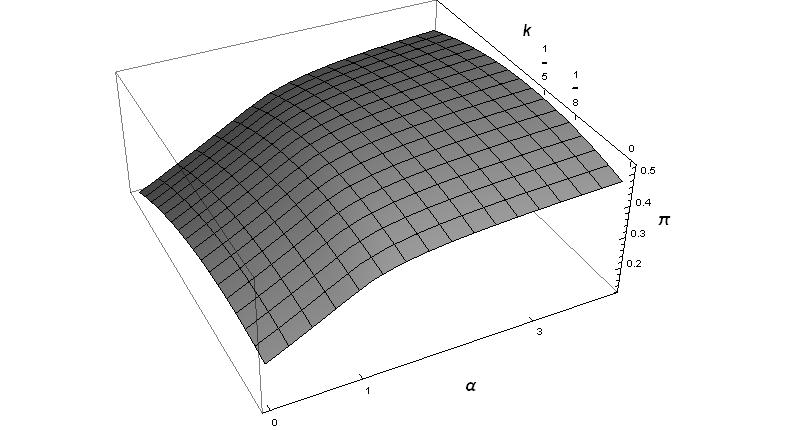
\includegraphics[width=1.0\textwidth]{./figures/Endogenousksimulation0.jpg}
\caption{Simulation of profits with a high cost of piracy }
\flabel{Classic case: Buyers and non-users, }
\label{endk1}
\end{figure}

Similarly we simulate the case where $0<r<\tilde{r}$. Since we now have an additional dimension to represent, we use a 3D contour graph, see figure \ref{endk2}. In this case the $k$ is the optimal k pursued. Notice that once again the equilibrium $k$ is around $\frac{1}{8}$ for low values of product degradation $r$. However, in this scenario, the previous result is reversed, that is, higher piracy pursuit decreases the optimal product improvement. The intuition behind this counterintuitive result is that $r$ and $k$ are substitutes, the firm can use the higher $r$ as an alternative to spending on $k$. In other words, the local effect of an increase in $r$ within $0<r<\tilde{r}$ is to decrease product improvement but once $r=\tilde{r}$, then there is a discontinous jump which depends on the network value which causes an increase in product improvement. 


\begin{figure}[t!] 
\centering
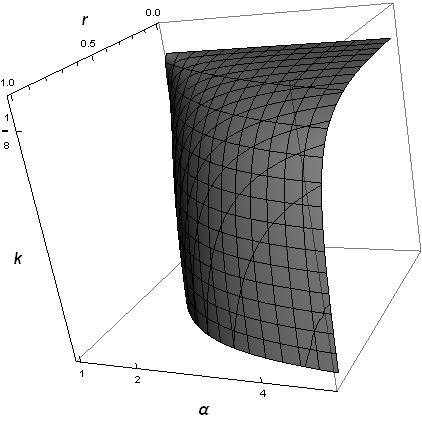
\includegraphics[width=0.5\textwidth]{./figures/Endogenousksimulation.jpg}
\caption{Intermediate cost of piracy case: Contour of the profit function maximized with repspect to the product improvement}
\flabel{Buyers, pirates and non-users}
\label{endk2}
\end{figure}


% In the classic case, where there are no pirates because the cost of piracy is high, the model becomes more complex and has no simple closed form solution for product improvement. If we fix the network value to be equal to base value of the product $\alpha=1+k$, we have that $\tilde{k} = \frac{1}{3 \sqrt{3}} \approx \frac{1}{5}$, numerically this is the highest product improvement that can be pursued, therefore product improvement is maximized when the network value is equal to the base value \footnote{Note that because the cost of product improvement is quadratic, the network value will increase faster than the product improvement, therefore at some point, the equality $\alpha = 1+k$ will hold. If we take the limit of the demand function, $1-\tilde{x}$ with $\alpha$ approaching this parameterization we have that the demand is $\frac{\sqrt{(1+k)(1+k-p)}}{1+k}$. Using this in the profit function, we attain that $p=\frac{2}{27} (9 + \sqrt{3})$ and $k=\frac{1}{3 \sqrt{3}} $ and consequently, profit is, $\pi = \frac{1}{27} \left(1+6 \sqrt{3}\right)$.}.

% In fact even if there is no network value the product improvement pursued is equal the value pursued in the cost-less case,  $\alpha=0 \Rightarrow \tilde{k} = \frac{1}{8}$. Numerically we can also see that as $\alpha$ approaches a large number, $k$ approaches $\frac{1}{9}$
% \footnote{even at $\alpha=100 000 000, k=.1111111$  }. Implying that product improvement peaks when network value is equal to base value. 


% \begin{proposition}
% \label{substitutabilityproposition}
% The network value is substituable with product improvement. 
% \end{proposition}

% \begin{proof}
% See appendix: \ref{substitutabilityproof}
% \end{proof}


% The extra first and second order conditions are given by:

% \begin{equation*}
% \frac{\partial \pi}{\partial k} = \frac{ p(p-r)}{((\alpha-1)
% \sqrt{ 1-r }
% +k)^2} -2k
% \end{equation*}

% \begin{equation*}
% \frac{\partial^2 \pi}{\partial k^2} = -\frac{2 p(p-r)}{((\alpha-1)
% \sqrt{ 1-r }
% +k)^3} -2
% \end{equation*}


% \begin{proposition}
% \label{alphak}
% If $\alpha>1$ then an increase in $\alpha$ can only decrease the pursued product improvement. 
% \end{proposition}

% \begin{proof}
% First we derive with respect to the exogenous variables. Due to the envelope theorem we need only look at the direct effects of the derivative and can ignore indirect effects due to the price. 
% \begin{equation*}
% \frac{\partial \pi }{\partial \alpha} =\frac{\sqrt{1-r}p^* (p^*-r)}{\left((a-1) \sqrt{1-r}+k\right)^2}
% \end{equation*}

% We then proceed to derive with respect to $k$:
% \begin{equation*}
% \frac{\partial^2 \pi }{\partial \alpha k} =
% -\frac{2 \sqrt{1-r} (p^*-r)}{\left((\alpha-1) \sqrt{1-r}+k\right)^3}
% \end{equation*}
% Since this derivative is negative if $\alpha>1$ and $p^*>r$ it implies substitutability between $\alpha$ and k.  
% \end{proof}

% The more intuitive interpretation of proposition \ref{alphak} is simply that the firm will invest to improve the product when the good has a low network value, but as the network value of the good increases, it no longer has need to undertake this investment and since investment is costly, it will just decrease the degree at which it is pursued.

% In the intermediate cost of piracy case, there is once again no closed form solution. Some point estimates, a first and second order approximations are done in the appendix notes(\ref{notes}). However we can deduce how the firm would optimize product improvement with respect to $\alpha$. 

% \begin{corollary}
% Proposition \ref{alphak} implies that the upper bound value of product improvement is $k= \frac{1}{8}$
% \end{corollary}


% To see this corollary we need only note if $\alpha$ was smaller than 1, then the derivative would be positive and therefore the two would be complementary. So the product improvement peaks a $\alpha=1$ and then starts to decrease. In other words, the product improvement pursued when there are no pirates is an upper bound on the intermediate piracy. The firm has a higher incentive to increase the value of its product if pirating is free. 

% \begin{proposition}
% If the network value is large, then further increases in the network value increases the number of buyers. 
% \end{proposition}

% \begin{proof}
% \begin{align*}
% 1 - \hat{x}= 1 - \frac{p-r}{(\alpha - 1) \sqrt{1-r} +k} \\
% = 1 - \frac{k+ (\alpha-1)\sqrt{ 1 -r }-r}{2(\alpha - 1) \sqrt{1-r} +2k} \\
% \frac{\partial (1 - \hat{x})}{\partial \alpha}=  -\frac{ \frac{\partial k}{\partial \alpha}+ \sqrt{ 1 -r }}{2(\alpha - 1) \sqrt{1-r} +2k}+\frac{(k+ (\alpha-1)\sqrt{ 1 -r }-r) (2 \sqrt{1-r}+\frac{\partial k}{\partial \alpha})}{(2(\alpha - 1) \sqrt{1-r} +2k)^2} \\
% =-\frac{\frac{\partial k}{\partial \alpha} \left(\alpha \sqrt{1-r}+k+r-\sqrt{1-r}\right)+2 r\sqrt{1-r} }{4 \left((\alpha-1) \sqrt{1-r}+k\right)^2}
% \end{align*}

% First note that from proposition \ref{alphak} we know that the derivative of k is negative, therefore the whole term is negative if:

% \begin{align*}
% \alpha \sqrt{1-r}+k+r-\sqrt{1-r}<0 \\
% \alpha <1-\frac{k+r}{\sqrt{1-r}}<1 
% \end{align*}

% The above condition never occurs. Because $\alpha>1$ by assumption. 

% We need only check the condition for which the left hand term of the numerator is larger than the right hand term. 
% \begin{align*}
% \alpha>\frac{2 r}{\frac{\partial k}{\partial \alpha}}-\frac{k}{\sqrt{1-r}}-\frac{r}{\sqrt{1-r}}+1 \\
% \end{align*}

% Note that since we know that when $\alpha$ is large, the effect on k approaches 0, this implies that the RHS approaches negative infinity, therefore $\alpha$ increases gradually the proportion of buyers
% \end{proof}

\section{Discussion and Conclusion}
The interpretation so far has been about network goods however a reputation interpretation could work equally well. If we interpret both $\alpha$ and $\beta$ as reputational effects. Both $\alpha$ and $\beta$ can be seen as signalling devices that can only be recognized by the portion of agents who are using. This interpretation may be less intuitive, however it more naturally explains why there may be a differential between the two network values.

The model has been assuming a kind of worse case scenario as to the effect of pirates. Though pirates can be used by the firm to increase its prices, there is no direct revenue mechanism for them. This could easily be imagined in a few cases, for instance, in the digital world a higher use base would allow for indirect profit opportunities. Take a social network as an example, a larger user base allows the network owner to sell advertising slots at a higher price, and the wider the reach the more profitable the enterprise. This kind of mechanism would only strengthen the profits of the firm in the pure piracy case whilist leaving the classic case unaffected. 

Welfare in the model is always decreasing with respect to the cost of piracy. This is simply because the firm mostly does not produce the product since the welfare from an increase in user base is always positive. In the baseline model the product already exists, it only by endogenizing the product improvement that the firm can add value. This does not entail that product degradation should always be zero because profits must be higher than the fixed cost of creating the product. Instead, it should only be noted that the framework presented here actually implies the existence of pareto improving policies. That is, when the network value is high the firm prefers there to be a higher amount of piracy over no piracy at all. 

% In the standard literature, the only source of revenue for a firm is to sell the product. However there are situations, especially in the digital world where having a larger user base also allows for additional indirect profit opportunities. For instance in a social network, a larger user base allows the network owner to sell advertising slots at a higher price, and the wider the reach the more profitable the enterprise. This extra source of revenue is parametrized with the letter $\lambda$. It should be noted that increasing pirates or buyers increase revenue from this source. 

Our model shows that even if the firm has total control of the level of piracy pursuit, it would not necessarily fully utilize this capability. Under the conditions discussed above, the firm often has incentive to not use deterrence to push consumers out of its pool of customers because reducing the number of consumers also decreases the value of the good for those who would buy. The intuition behind this carrot and stick approach is that the price has a single effect whilst piracy pursuit has a double effect. The price effect is less variable because it gives the firm the ability to be more precise in its targeting mechanism. Wile changing the price only works on the consumers who are marginally on the edge of the choice of buying or pirating, changing the degradation level affects all segments at once, resulting in more global network effects. 

Increasing the product degradation affects both the proportion of users buying while also decreasing the user base. The strength of these two effects depends on their valuation of the network value. The decrease in the user base corresponds to the product becoming less popular and the change in buying behavior represents either a consumer who no longer wishes to undertake the risk of pirating or a consumer who no longer wishes to buy the product because it has less value to her.

Though the more traditional way of seeing pirates is as a competitive force, in the model presented here pirates take the role of the path of least resistance. Indeed controlling the pirates to ensure that they are at the right level is a fine art and the if the instrument is too blunt, it may cause more harm than good. The conditions for piracy to be optimal are relatively mild, the bought network value need only reach a certain threshold for it to be worthwhile. Indeed though the model assumed that pursuing pirates is costless, in the real world, there are significant costs both from the point of view of the planner and the firm. The endogenization of these costs would only decrease the threshold $\alpha$ for which the firm would prefer piracy to exist.

One simple policy implication of the model is that pursuing pirates uniformly for all their activities may have welfare reducing effects. An optimal solution would be one where the pursuit of piracy is  heterogeneous to each firm. Much like how firms only sue specific infringers and let others go, the same can be encouraged on the consumer side. From the legal point of view the implication is that piracy could be viewed as a civil or corporate issue and not a criminal one. For broadening the scope of tort law, see \citep{DF96}. 

Still, this approach is limited in that, whilst it is possible for a firm to identify other infringers and selectively sue them, it is likely that the number of pirates is too high to accurately identify. However, if we are to include the cost of identification, this same cost has to be applied on any mechanism that enforces piracy laws. A policy that focuses on enforcement against consumers is likely to have a much higher social cost than one which is enforced on firms in accordance with the actual number of consumers. 

Put in another way, the problem with copyright enforcement is that it is unconditional. That is, unlike patents, where the patent right holder chooses to initiate an action against a patent infringer, presumably following a calculation which leads the patent right holder to the conclusion that such an action is worthwhile. The illegal act of piracy is unconditionally a criminal offense. In other words, regardless of whether the effects of the act aid or harm a copyright owner there is a consistent social cost imposed. 

In practice, firms cannot control the probability of success when initiating an action. In industries where the pirates are many and are highly decentralized, it is quite plausible that neither the government nor the firms can greatly increase their level of piracy pursuit without greatly invading personal data and privacy laws. Realistically, cases involving music or movies are more adapted and fit better into the above developed model. 

It is also important to note that there are firm adaptation which can be used as alternatives to the law. These strategies may be less costly because they can focus on prevention rather than pursuit. In the digital space, these strategies are usually labeled, Digital Rights Management (DRM) strategies. Examples of DRM are idea's such as requiring users to use specific platforms to access the content, monitoring consumption, selling restricted usage copies etc. Such strategies may be complementary or substitutable with piracy enforcement. DRM strategies allow firms to select their own level of piracy pursuit. Piracy often has its own platforms which continously improve their own services. Indeed much of the historic incentive to pirate was due to the superior platform services of piracy software. The new wave of streaming services such as Netflix or Amazon prime represent competition to these piracy services.


A hidden assumption in the model presented above is that all users value socializing with all other users. In the real world, if there are segregation effects, this assumption may not be fully applicable. On the other hand, if we assume that segregation brings together more diverse valuations, such as perhaps a family unit, then this solidifies the conclusions of this model.

Generally, the assumption that utilities are independent is often too readily used. What is termed a "network good" in the industrial organization literature can be interpreted too narrowly. It is not simply digital social networks that have this property. In fact, it is possible to envision most goods as having both an intrinsic value and an extrinsic component. The relative ratio of intrinsic to extrinsic value will likely vary substantially between cultures, space and time. Additionally, the domain in which this is true is likely to extend much farther than what common intuition would entail. For instance, even perishable goods, such as food, are not necessarily exempt from this feedback process, for instance the consumption of cheese or wine is not something that is independent of the surrounding culture. Accordingly, much of what can be deemed "group identity" can be represented within a network good framework. A culture of baguette or chocolate eaters does not represent the same profit opportunities as groups without such culture.

One of the most common arguments against piracy is that it decreases the number of individuals who actually pay the real cost of the product.  However, the implicit assumption in such a line of reasoning is that the number of purchasers and the value of the purchasing, are independent. Based on the model presented here, such a conclusion is drawn too hastily, the effect of increasing the piracy cost may not have the desired effect. As pointed out in \cite{CRP91} this setup raises strange ethical questions. When we have possible parameter values that imply that higher pursuit of pirates may be worse for consumers and producers at public cost. With these factors in mind, it is unclear whether enforcing intellectual property rights passes even the most basic cost benefit analysis.

\newpage
\section{Appendix}
% \subsection{Buyers and pirates}
% \begin{equation*}
% \hat{x} = \frac{p}{\alpha-\beta + k}
% \end{equation*}

% The upper condition is $\alpha-\beta+k \geq p$. Therefore the price is:

% \begin{equation*}
% p = \frac{1}{2}\left(
% \alpha-\beta+k
% \right)
% \end{equation*}

% Note that these values imply that $\hat{x} = \frac{1}{2}$ regardless of the values of $\beta$ or $\alpha$. Profit is then:
% \begin{align*}
% \pi &= p(1-\hat{x}) \\
% &=  \frac{1}{4}\left(
% \alpha-\beta+k
% \right)  \\
% \end{align*}

% Social Surplus and welfare are:
% \begin{align*}
% \hat{S} &= \int_0^{\hat{x}}x(1+\beta)dx+
% \int_{\hat{x}}^{1}\left( x(1+\alpha+k)-p \right)dx \\
% &= \frac{1}{8} (\alpha+2 \beta+k+3) \\
% \hat{W} &= \frac{3}{8} \left( 1 + \alpha +k
% \right)
% \end{align*}



\subsection{Proof of proposition \ref{buyersusersprice}} \label{buyersuserspriceproof}

\begin{align*}
\textbf{The demand function in the case of buyers only is given by:} \\
1-\frac{\alpha+k+1-\sqrt{(-\alpha-k-1)^2-4 \alpha p}}{2 \alpha} \\
\frac{\alpha-k-1+\sqrt{(-\alpha-k-1)^2-4 \alpha p}}{2 \alpha}
\\
\textbf{The profit function is then:} 
\\
p*\frac{\alpha-k-1+\sqrt{(-\alpha-k-1)^2-4 \alpha p}}{2 \alpha}
\\
\text{Derivative with respect to p}: \\
\frac{\sqrt{(\alpha+k+1)^2-4 \alpha p}+\alpha-k-1}{2 \alpha}-\frac{p}{\sqrt{(\alpha+k+1)^2-4 \alpha p}} =0
% \\
% \frac{\sqrt{(\alpha+k+1)^2-4 \alpha p}+\alpha-k-1}{2 \alpha} =\frac{p}{\sqrt{(\alpha+k+1)^2-4 \alpha p}} \\
% %%%%%%%%%%%%%%%%%%%%%%%%%%%%%%%%%%%
% ( \alpha+k+1)^2-4 \alpha p+(\alpha-k-1)\sqrt{(\alpha+k+1)^2-4 \alpha p} = 2 p \alpha \\
% ( \alpha+k+1)^2+(\alpha-k-1)\sqrt{(\alpha+k+1)^2-4 \alpha p} = 6 p \alpha \\
% %%%%%%%%%%%%%%%%%%%%%%%%%%%%%%%%%%%%%
% (\alpha-k-1)\sqrt{(\alpha+k+1)^2-4 \alpha p} = 6 p \alpha - ( \alpha+k+1)^2 \\
% %%%%%%%%%%%%%%%%%%%%%%%%%%%%%%%%%%%
% (\alpha-k-1)^2((\alpha+k+1)^2-4 \alpha p) = (6 p \alpha - ( \alpha+k+1)^2 )^2
%%%%%%%%%%%%%%%%%%%%%%%%%%%%%
% \\
% (\alpha-k-1)^2(\alpha+k+1)^2-(\alpha-k-1)^2 4 \alpha p = 36 p^2 \alpha^2 + ( \alpha+k+1)^4 - 12 p \alpha ( \alpha+k+1)^2 
% \\
% 0 = 36 p^2 \alpha^2  +4 p \alpha((\alpha-k-1)^2-3( \alpha+k+1)^2) + ( \alpha+k+1)^2(( \alpha+k+1)^2-(\alpha-k-1)^2)
% \\
% 0 = 36 p^2 \alpha^2  +4 p \alpha((\alpha-k-1)^2-3( \alpha+k+1)^2) + ( \alpha+k+1)^2(4 \alpha(1+k))
\\
0 = 9 p^2 \alpha  -2 p (\alpha^2 + 4\alpha(1+k)+(1+k)^2) + ( \alpha+k+1)^2 (1+k)
\\
\textbf{This is gives two solutions for p:} \\
% \tilde{p} = \frac{(\alpha+k+1)^2+2\alpha(k+1) \pm \sqrt{(1-\alpha+k)^2(\alpha^2+\alpha (k+1)+(k+1)^2)}}{9 \alpha} \\
\tilde{p} = \frac{(\alpha+k+1)^2}{9 \alpha}+\frac{2(1+k)}{9}+\frac{ \pm \sqrt{(1-\alpha+k)^2(\alpha^2+\alpha (k+1)+(k+1)^2)}}{9 \alpha} \\
\end{align*}



\subsection{Corollaries of prop \ref{corollary1}, approximation and proportion} \label{corollary1proof}

If $\alpha$ is large relative to $1+k$, the expression simplifies, we will represent the use of this assumption by $\approx$. 

\begin{align*}
p \approx \frac{\alpha}{9}+\frac{2(1+k)}{9}+\frac{ \pm \sqrt{(\alpha^2+\alpha (k+1))}}{9 } \\
=\frac{\alpha}{9}+\frac{2(1+k)}{9}+\frac{ \pm \sqrt{(\alpha^2+\alpha^2 \frac{(k+1)}{\alpha})}}{9 } \\
=\frac{\alpha}{9}+\frac{2(1+k)}{9}+\frac{ \pm \alpha \sqrt{ \frac{k+1+\alpha}{\alpha}}}{9} \\
=\frac{2\alpha}{9}+\frac{2(1+k)}{9}
\end{align*}

\begin{align*}
&\sqrt{(\alpha+k+1)^2-4 \alpha p} \\
&\text{Substitute in the approximated price:} \\
&\approx\frac{1}{3} \sqrt{a^2+10 a (k+1)+9 (k+1)^2} \\
&\approx \frac{1}{3} \sqrt{a^2+10  \frac{a^2}{a} (k+1)} \\
&\approx \frac{a}{3} \sqrt{1+ \frac{10}{a} (k+1)} \\
&\approx  \frac{a}{3}
\end{align*}

We can use this expression to represent the proportion of agents who will consume in equilibrium:

\begin{align}
1-\tilde{x} &= 1-\frac{\alpha+k+1-\frac{a}{3}}{2 \alpha} \\
&=\frac{4\alpha-3(1+k)}{6\alpha}
\approx \frac{2}{3}
\end{align}


\subsection{Proof of proposition \ref{piracyvsnotproposition}}\label{piracyvsnot}

We now look at the what the derivative of the profit function turns out to be. First note that in proposition \ref{envelopetheorem} we deduce that the envelope theorem applies. We also use corollary \ref{corollary1} to simplify the square root to have the simplified price which assumes that $\alpha$ is large. 

\begin{align*}
\frac{\partial f}{\partial \alpha} &= \frac{\frac{2 (\alpha+k+1)-4 p}{2 \sqrt{(\alpha+k+1)^2-4 \alpha p}}+1}{2
   \alpha}-\frac{\sqrt{(\alpha+k+1)^2-4 \alpha p}+\alpha-k-1}{2 \alpha^2} \\
% =\frac{1}{2 \alpha}
% \left( 
% \frac{2 (\alpha+k+1)-4 p}{2 \sqrt{(\alpha+k+1)^2-4 \alpha p}}+1-\frac{\sqrt{(\alpha+k+1)^2-4 \alpha p}+\alpha-k-1}{ \alpha}
% \right) \\
% =\frac{1}{2 \alpha}
% \left( 
% \frac{ (\alpha+k+1)-2 p}{ \sqrt{(\alpha+k+1)^2-4 \alpha p}}-\frac{\sqrt{(\alpha+k+1)^2-4 \alpha p}-k-1}{ \alpha}
% \right) \\
% =\frac{1}{2 \alpha}
% \left( 
% \frac{ \alpha (\alpha+k+1)-2 \alpha p}{ \alpha\sqrt{(\alpha+k+1)^2-4 \alpha p}}-\frac{\sqrt{(\alpha+k+1)^2-4 \alpha p}(\sqrt{(\alpha+k+1)^2-4 \alpha p}-k-1)}{ \alpha\sqrt{(\alpha+k+1)^2-4 \alpha p}}
% \right) \\
% =\frac{1}{2 \alpha}
% \left( 
% \frac{ \alpha (\alpha+k+1)-2 \alpha p}{ \alpha\sqrt{(\alpha+k+1)^2-4 \alpha p}}-\frac{\sqrt{(\alpha+k+1)^2-4 \alpha p}(\sqrt{(\alpha+k+1)^2-4 \alpha p}-k-1)}{ \alpha\sqrt{(\alpha+k+1)^2-4 \alpha p}}
% \right) \\
% =\frac{1}{2 \alpha^2 \sqrt{(\alpha+k+1)^2-4 \alpha p}}
% \left( 
% \alpha (\alpha+k+1)-2 \alpha p-\sqrt{(\alpha+k+1)^2-4 \alpha p}(\sqrt{(\alpha+k+1)^2-4 \alpha p}+k+1)
% \right) \\
% =\frac{1}{2 \alpha^2 \sqrt{(\alpha+k+1)^2-4 \alpha p}}
% \left( 
% \alpha (\alpha+k+1)-2 \alpha p-(\alpha+k+1)^2+4 \alpha p+(k+1)\sqrt{(\alpha+k+1)^2-4 \alpha p})
% \right) \\
% =\frac{1}{2 \alpha^2 \sqrt{(\alpha+k+1)^2-4 \alpha p}}
% \left( 
% \alpha (\alpha+k+1)-(\alpha+k+1)^2+2 \alpha p+(k+1)\sqrt{(\alpha+k+1)^2-4 \alpha p})
% \right) \\
% =\frac{1}{2 \alpha^2 \sqrt{(\alpha+k+1)^2-4 \alpha p}}
% \left( 
% -(1+k)(\alpha+k+1)^2+2 \alpha p+(k+1)\sqrt{(\alpha+k+1)^2-4 \alpha p})
% \right) \\
&=\frac{1}{2 \alpha^2 \sqrt{(\alpha+k+1)^2-4 \alpha p}}
\left( 
2 \alpha p+(k+1)(\sqrt{(\alpha+k+1)^2-4 \alpha p})-(\alpha+k+1)^2)
\right) \\
\end{align*}


% \ref{corollary1proof}

\begin{align*}
\textbf{We now assume that $\alpha$ is large relative to k+1 and substitute in the price and square root}
\\
=\frac{3}{2 \alpha^3 }
\left( 
2 \alpha p+(k+1)(\frac{a}{3}-(\alpha+k+1)^2)
\right) \\
=\frac{3}{2 \alpha^3 }
\left( 
2 \alpha (\frac{2\alpha}{9}+\frac{2(1+k)}{9})+(k+1)(\frac{a}{3}-(\alpha+k+1)^2)
\right)
\\
=\frac{3}{2 \alpha^3 }
\left( 
\frac{4\alpha^2}{9}+\frac{4\alpha(1+k)}{9}+(k+1)(\frac{a}{3}-(\alpha+k+1)^2)
\right)\\
=\frac{3}{18 \alpha^3 }
\left( 
4\alpha^2+4\alpha(1+k)+(k+1)(\frac{a}{3}-(\alpha+k+1)^2)
\right)\\
\textbf{Multiply by the price}
\\
p(a)\frac{\partial f}{\partial \alpha} = (\frac{2\alpha}{9}+\frac{2(1+k)}{9})\frac{3}{18 \alpha^3 }
\left( 
4\alpha^2+4\alpha(1+k)+(k+1)(\frac{a}{3}-(\alpha+k+1)^2)
\right)\\
= \frac{\alpha +1+k}{27 \alpha^3 }
\left( 
4\alpha^2+4\alpha(1+k)+(k+1)(\frac{a}{3}-(\alpha+k+1)^2)
\right)
\\
= \frac{\alpha +1+k}{27 \alpha^3 }
\left( 
4\alpha^2+(k+1)(\frac{13a}{3}-(\alpha+k+1)^2)
\right)\\
\end{align*}

\begin{align*}
\text{If alpha is large relative to k+1}\\
= \frac{\alpha}{27 \alpha^3 }
\left( 
4\alpha^2+(k+1)(\frac{13a}{3}-\alpha^2)
\right)
\\
= \frac{1}{27 \alpha^2 }
\left( 
4\alpha^2+(k+1)(\frac{13a}{3}-\alpha^2)
\right) \\
= \frac{1}{27 \alpha^2 }
\left( 
4\alpha^2+(k+1)\frac{\alpha}{3}(13-3 \alpha)
\right)
\\
= \frac{1}{71 \alpha }
\left( 
12\alpha+(k+1)(13-3 \alpha)
\right) \\
\text{If the second term is negative, which occurs after $\alpha$ exceeds 5 we can say}
\\
= \frac{1}{71 \alpha }
\left( 
12\alpha+(k+1)(13-3 \alpha)
\right) < \frac{12}{71 }
\end{align*}
Recall that the slope of the profit function with pirates is $\frac{1}{4}$, therefore profit under piracy increases more than profit without piracy if $\alpha$ is relatively large


% \subsection{Proof of proposition \ref{substitutabilityproposition} }

% \label{substitutabilityproof}

% \begin{proof}
% First note that the cross partial derivative is given by:
% \begin{equation*}
% \frac{\partial^2 \pi}{\partial \alpha k} =
% \frac{p \left(-\frac{\alpha+k+1}{\sqrt{(\alpha+k+1)^2-4 \alpha p}}-\frac{2 \alpha p (\alpha-k-1)}{\left((\alpha+k+1)^2-4 \alpha p\right)^{3/2}}+1\right)}{2 \alpha^2} 
% \end{equation*}

% To check the sign we need only see that the two first terms inside the parenthesis are decreasing in $\alpha$. 
% \begin{align*}
% &= \left(-\frac{\alpha+k+1}{\sqrt{(\alpha+k+1)^2-4 \alpha p}}-\frac{2 \alpha p (\alpha-k-1)}{\left((\alpha+k+1)^2-4 \alpha p\right)^{3/2}}+1\right)&& \\
% %%%%%%%%%%%%%%%%%%%%%%%%%%%%%%%%%
% &= 1- \frac{2 \alpha p (\alpha-k-1)+((\alpha+k+1)^2-4 \alpha p)(1+k+\alpha)}{\left((\alpha+k+1)^2-4 \alpha p\right)^{3/2}}& \\
% %%%%%%%%%%%%%%%%%%%%%%%%%%%%%%%%%
% &= \frac{\left((\alpha+k+1)^2-4 \alpha p\right)^{3/2}-2 \alpha p (\alpha-k-1)-((\alpha+k+1)^2-4 \alpha p)(1+k+\alpha)}{\left((\alpha+k+1)^2-4 \alpha p\right)^{3/2}}& \\
% %%%%%%%%%%%%%%%%%%%%%%%%%%%%%%%%%
% &=\frac{\left((\alpha+k+1)^2-4 \alpha p\right)^{3/2}+2 \alpha p (\alpha-3(k+1))-((\alpha+k+1)^3}{\left((\alpha+k+1)^2-4 \alpha p\right)^{3/2}} &
% \end{align*}*

% Note that if $\alpha=0$ then the cross partial is 0. Then note that in the last expression, the last term is always larger than the first term when $k>0,\alpha>0, p>0$. Then note that the second term is negative whenever $\alpha<3$ and if $\alpha>3$ then the cube route effect of the last term dominates.  
% \end{proof}

\subsection{Proof of proposition \ref{tdemand}}

\label{tdemandp}

We first begin with the condition which renders an agents indifferent between pirating and not using to solve for the valuation $x$ of the indifferent pirate. 


\begin{align*}
x(1+\beta(1-F(x)))-r=0 \\
x(1+\beta(1-x))=0 \\
x+x\beta-\beta x^2-r=0 \\
x^2-x\frac{(1+\beta)}{\beta} +\frac{r}{\beta} = 0 \\
\check{x} = \frac{(1+\beta)}{2 \beta}
\pm
\frac{ \sqrt{ \left(\frac{(1+\beta)}{\beta}\right)^2 -4\frac{r}{\beta} } }{2} \\
\check{x} = \frac{(1+\beta)}{2 \beta}
\pm
\frac{ \sqrt{ \left(1+\beta\right)^2 -4r\beta } }{2 \beta} \\
\end{align*}



\begin{equation*}
\check{x} = 1
\pm \sqrt{ 1 -r }
\end{equation*}

If $\check{x}>1$ is verified this implies that no users will be pirating since all users prefer not to pirate. Therefore only the negative solution can be used.  With the indifferent user, we need only take the difference $1-\check{x}$ to know the proportion of agents who are users. This proportion is simply:

\begin{align*}
1-\check{x}=\sqrt{ 1 -r }
\end{align*}

We note that the proportion of agents who are users is entirely exogenous to the firm. What is endogenous to the firm is the proportion of agents who are buyers. The proportion of agents who are buyers, ceteris parabus, depends on the proportion who are pirates. The consumer who is indifferent between purchasing and pirating can similarly be found by equating the two options. Which gives the following value:

\begin{align*}
x(1+\beta(1-F(x)))-r=x(1+\alpha(1-F(x)))-p \\
\Rightarrow \hat{x}=\frac{p-r}{(\alpha-1)\sqrt{ 1 -r }+k} \\
\end{align*}

Where the last step occurs because $1-F(x)=1-\check{x}$. Recall that $\hat{x} \geq \check{x}$ from the preliminary section. The demand function for buying can then simply be written as:

\begin{align*}
D(\hat{x})=1-\hat{x}=1-\frac{ (p-r)}{k + (\alpha-1) \sqrt{ 1 -r }} \\
%%%%%%%%%%%%%%%%%%%%%%%%%%%%%%%%
\frac{\partial D(\hat{x})}{\partial p} =
-\frac{ 1}{k + (\alpha-1) \sqrt{ 1 -r }} \\
%%%%%%%%%%%%%%%%%%%%%%%%%%%%%%%%%
\frac{\partial D(\hat{x})}{\partial k} =
\frac{ (p-r) }{(k+
 (\alpha-1)\sqrt{ 1 - r }
)^2} 
%%%%%%%%%%%%%%%%%%%%%%%%%%%%%%%%%
%%%%%%%%%%%%%%%%%%%%%
\end{align*}

% This condition must satisfy that the higher indifferent agent must have a lower valuation, $x$ than the highest valuation user, $\hat{x} \leq 1$. This constraint can be used to give us an upper bound on the price the firm can charge. We call this condition 1, $C_1$

% \begin{align*}
% \hat{x} \leq 1 \\
% \frac{p-r}{(\alpha-1)\sqrt{ 1 -r }+k} \leq 1
% \\
% p \leq (\alpha-1)\sqrt{ 1 -r }+k+r \\
% \text{or we can get an upper bound on k} \\
% p -(\alpha-1)\sqrt{ 1 -r } -r\leq k \\
% \text{similarly we can use the lower bound:} \\
% \hat{x} \geq 0 \\
% \frac{p-r}{(\alpha-1)\sqrt{ 1 -r }+k}  \geq 0 \\
% p \geq r
% \end{align*}

% We similarly recall that the indifferent consumer between buying and pirating must be higher than the indifferent consumer between pirating and not buying, $\hat{x}>\check{x}$. We can use this condition to get a further condition.  We call this the second condition $C_2$
% \begin{align*}
% C_2 = \frac{p-r}{(\alpha-1)\sqrt{ 1 -r }+k} -\sqrt{ 1 -r } \geq 0
% \\
% \frac{p-r}{(\alpha-1)\sqrt{ 1 -r }+k} 
% \geq
% \sqrt{ 1 -r } \\
% p-r
% \geq \sqrt{ 1 -r }((\alpha-1)\sqrt{ 1 -r }+k) \\
% p-r
% \geq (\alpha-1)( 1 -r )+k\sqrt{ 1 -r } \\
% p
% \geq \alpha -1+r(2-\alpha)+k\sqrt{ 1 -r }
% \end{align*}

% We can compare this constraint to the previous one to see that this one is stricter:

% \begin{align*}
% -1+r(2-\alpha)+k\sqrt{ 1 -r } \geq r \\
% \Rightarrow
% k\sqrt{ 1 -r } + (1 -r)(\alpha-1) \geq 0
% \end{align*}








\section{Endogenous k}


\subsection{case where $r=0$}

\begin{proposition}
If $r=0$, the firm will choose $(p,k)=(\frac{1}{16c}+\frac{\alpha-\beta}{2},\frac{1}{8c})$ $\check{x}=0$ and $\hat{x}=1/2$ and $\pi= \frac{1}{4}(\alpha-\beta)+\frac{1}{64c}$.
\end{proposition}

\begin{proof}


As in the exogenous case we solve for the indifference condition:

\begin{align*}
\hat{x}(1+\alpha+k)=\hat{x}(1+\beta) \\
\Rightarrow \hat{x} = \frac{p}{\alpha - \beta +k}
\end{align*}


Now, the profit function is

\begin{equation*}
\tilde{\pi} = p\left(1-\frac{p}{\alpha - \beta +k}\right)-c k^2
\end{equation*}

The two first order conditions, relatives to $p$ and $k$, for the profit maximization are:

\begin{align*}
\frac{\partial \tilde{\pi}}{\partial p}= 1-\frac{2p}{\alpha - \beta +k}\\
\frac{\partial \tilde{\pi}}{\partial k}=  \frac{p^2}{(\alpha-\beta+k)^2}-2ck 
\end{align*} 

\begin{equation*}
p = \frac{\alpha-\beta-k}{2}
\end{equation*}

and 

\begin{equation*}
2ck = \frac{p^2}{(\alpha-\beta+k)^2}
\end{equation*}

This gives $k^*=\frac{1}{8c}$,  and $p^*=\frac{\alpha-\beta}{2}+\frac{1}{16c}$ and $\pi=\frac{1}{4}(\alpha-\beta)+\frac{1}{64c} $ if we put these values in the profit equation. 

\end{proof}

\begin{observation}
The product improvement chosen by the firm does not depend on network values, $\beta$ and $\alpha$
\end{observation}


\subsection{Intermediate r}
$0<r<\tilde{r}$

We need to also verify that the profit function satisfies the first and second order conditions with respect to the price level.

\begin{align*}
\pi = p\left(1-\hat{x}\right) - k^2 \\
%%%%%%%%%%%%%%%%%%%%%
=p\left(1-\frac{ (p-r)}{(\alpha-1)
\sqrt{ 1-r }
+k} \right) -k^2
\\
%%%%%%%%%%%%%%%%%%%%%
\frac{\partial \pi }{\partial p} = 1-\frac{ (2p-r)}{
k+ (\alpha-1)\sqrt{ 1 -r }} \\
%%%%%%%%%%%%%%%%%%%%%
\frac{\partial^2 \pi }{\partial p^2}
= -\frac{ 2}{
k+ (\alpha-1)\sqrt{ 1 -r }} \\
%%%%%%%%%%%%%%%%%%%%%
%%%%%%%%%%%%%%%%%%%%%
%%%%%%%%%%%%%%%%%%%%%
\frac{\partial \pi}{\partial k} = \frac{ p(p-r)}{((\alpha-1)
\sqrt{ 1-r }
+k)^2} -2k
\\
%%%%%%%%%%%%%%%%%%%%%
\frac{\partial^2 \pi}{\partial k^2} = -\frac{2 p(p-r)}{((\alpha-1)
\sqrt{ 1-r }
+k)^3} -2 
\end{align*}

\subsection{Some values for k}

We now set $ (\alpha-1)\sqrt{ 1 -r }=w$ and proceed to solve for $k$ using the second FOC.  

\begin{align*}
\frac{\partial \pi}{\partial k} = \frac{ p(p-r)}{(w
+k)^2} -2k \\
2k= \frac{ p(p-r)}{(w
+k)^2} \\
2k(w+k)^2=p(p-r) \\
\text{We now substitute the price into the this: } \\
2k(w+k)^2=\frac{k+ w+r}{2} \left(\frac{k+ w+r}{2}-r \right) \\
2k(w+k)^2=\frac{k+ w+r}{2} \left(\frac{k+ w-r}{2} \right) \\
8k(w+k)^2= \left( k+ w+r \right) \left(k+ w-r\right) \\
\text{If we assume that $w=r$} \\
\Rightarrow 
k = \frac{1}{16} \left(1\pm \sqrt{32 r+1}\right) - r\\
\text{Only the positive solution yields positive values} \\
= \frac{1}{16} \left(1\pm \sqrt{32 r+1}\right) - r \\
\text{This function is maximized at $k=\frac{1}{8}$} \\
\text{We now take a limit case as $\alpha$ increases:} \\
8k(w+k)^2= \left( w+ k \right)^2 \\
k = \frac{1}{8} \\
\text{Similarly if:} \\
\alpha=1=\beta \\
\Rightarrow w = 0 \\
\Rightarrow k = \frac{1}{8} 
\end{align*}

\subsection{Notes} \label{notes}

\subsubsection{Why the envelope theorem applies} \label{envelopetheorem}


For notational simplicity we represent the demand function which is a function of $\alpha, p, k$ as $l(a, k(a),p(a))$.  

\begin{align*}
\pi(a, p(a),k(a))= p(a) l(a, k(a),p(a))-k(a)^2 \\
%%%%%%%%%%%%%%%%%%%%%%%%%%%%%%%%
\frac{ \partial \pi(a, p(a),k(a))}{\partial \alpha}= \frac{\partial p(a) }{\partial a } \left(
l(a, k(a),p(a)) \right)
+ p(a)\left( \frac{\partial l}{\partial a}
+\frac{\partial l}{\partial k(a)}\frac{\partial k(a)}{\partial a}
+\frac{\partial l}{\partial p(a)}\frac{\partial p(a)}{\partial a}
\right)
- 2 k(a) \frac{\partial k(a)}{\partial a}
\\ 
%%%%%%%%%%%%%%%%%%%%%%%%%%%
= \frac{\partial p(a) }{\partial a } \left(
l(a, k(a),p(a)) +p(a) \frac{\partial l}{\partial p(a)} \right)
+ p(a) \frac{\partial l}{\partial a}
+\frac{\partial k(a)}{\partial a}\left( p(a)\frac{\partial l}{\partial k(a)}-2 k(a)
 \right) \\
FOCS: 
\\
\frac{\partial \pi(a, p(a),k(a))}{\partial p(a)}=l(a, k(a),p(a))+p(a) \frac{\partial l}{\partial p(a)}=0 
\\
\frac{\partial \pi(a, p(a),k(a))}{\partial k(a)}=p(a) \frac{\partial l}{\partial k(a)} -2 k(a)=0
\\
\textbf{applying the FOC's we can simplify to}
\\
\frac{ \partial \pi(a, p(a),k(a))}{\partial \alpha}= 
p(a) \frac{\partial l}{\partial a} \\
\end{align*}

Therefore we can deduce the effects of $\alpha$ by simply taking the direct derivative of the profit function. The argument is equivalent for $r$.

\subsubsection{Regularly varying functions}\label{regul}

\begin{definition}
A regularly varyng function $L: (0,+ \infty) \rightarrow (0,+ \infty)$ has the following property:
\begin{equation}
lim_{x \rightarrow \infty} \frac{L(t x)}{L(x)} = g(t)
\end{equation}
\end{definition}

It is known that in regular varying functions, $g(t)$ take the following form\citep{bojanic1963slowly}:
\begin{equation}
g(t)=t^i
\end{equation}

If $g(t)= t$ this implies that the function is eventually linear. 

\begin{align}
L(x)-L(a x) = L(x) - f(a)L(x) = L(x)(1-f(a)) \\
L(y)-L(b y) = L(y) - f(b)L(y) = L(y)(1-f(b)) \\
\text{Linearity  implies:}
x-ax = y-yb \\
\rightarrow y = x \frac{(1-a)}{(1-b)} \\
\rightarrow L\left(x \frac{1-a}{1-b}\right)[1-f(b)] \\
\rightarrow f\left( \frac{1-a}{1-b}\right)L(x)[1-f(b)] \\
\text{L is linear in x if} \\
L(x)f\left(\frac{1-a}{1-b}\right)(1-f(b)) = L(x)(1-f(a)) \\
f\left(\frac{1-a}{1-b} \right) = \frac{1-f(a)}{1-f(b)} \\
\left(\frac{1-a}{1-b} \right)^i = \frac{1-a^i}{1-b^i} 
\end{align}

Which is satisfied because $g(t)=t$ implies $i=1$

\subsubsection{Welfare}

Welfare is just the sum of the social surplus and the profit.

\begin{align*}
W_{bn} = \int^{\tilde{x}}_0 \left(x(1+\alpha(1-\tilde{x})+\tilde{k})-\tilde{p} \right) dx + \tilde{\pi}  \\
W_{bp} = \int^{\hat{x}}_0 x(1+\beta) dx +\int^{1}_{\hat{x}} \left(x(1+\alpha+\hat{k}) - \hat{p} \right) dx + \hat{\pi} \\
W_{bpn} =
\int^{\hat{x}}_{\check{x}} \left(x(1+\beta(1-\check{x}))-r \right)dx +\int^{1}_{\hat{x}} \left(x(1+\alpha(1-\check{x})+\check{k}) - \check{p} \right) dx + \check{\pi}
\end{align*}

% \subsubsection{First and second order approximations of endogenous k}

% \begin{align*}
% \text{If we don't take the limit case then this is:} \\
% 8k(w+k)^2= \left( w+k \right)^2 -r^2 \\
% (w+k)^2(8k-1)=-r^2 \\
% \text{If we take a first order approximation:} \\
% f(k)= (w+k)^2(8k-1)+r^2 
% \\
% \approx f(t)+f'(t)(k-t) \\
% =(8 t-1) (t+w)^2+r^2 
% +(8 (t+w)^2+2 (8 t-1) (t+w))(k-t) \\
% \Rightarrow k = \frac{2 t+w^2+2 w-15 t^2-14 t w-r^2}{8 (t+w)^2}
% \\
% \text{If we approximate around $t=\frac{1}{8}$} \\
% k = \frac{(8 w+1)^2-64 r^2}{8 (8 w+1)^2} 
% \\
% \text{If we approximate around $t=0$} \\
% k= \frac{w (w+2)-r^2}{8 w^2}
% \\
% \text{So k is decreasing with r} \\
% \end{align*}

% \begin{align*}
% \text{A second order approximation of the function:} \\ 
% f(k)= (w+k)^2(8k-1)+r^2 \\
% \approx f(t)+f'(t)(k-t)+\frac{f''(\alpha)}{2}(k-t)^2 \\
% = (8 t-1) (t+w)^2+r^2 
% +(8 (t+w)^2+2 (8 t-1) (t+w))(k-t) \\
% +\frac{32 (t+w)+2 (8 t-1)}{2}(k-t)^2 \\
% = (8 t-1) (t+w)^2+r^2 
% +(8 (t+w)^2+2 (8 t-1) (t+w))(k-t) \\
% +(16 (t+w)+ (8 t-1))(k-t)^2 
% \end{align*}



% %\begin{equation*}
% %k = \frac{\pm \sqrt{\left(2 t-40 t^2-16 %t w+8 w^2\right)^2-4 (24 t+16 w-1) %\left(r^2+24 t^3+16 t^2 w+14 t^2+14 t %w-2 t-w^2-2 w\right)}+40 t^2+16 t w-2 %t-8 w^2}{2(24 t+16 w-1)} 
% %\end{equation*}
% We solve for k around 0: 

% \begin{align*}
% k = \frac{\pm \sqrt{\left(8 w^2\right)^2-4 (16 w-1) \left(r^2-w^2-2 w\right)}-8 w^2}{2(16 w-1)} \\
% =\frac{\pm 2 \sqrt{16 w^4- (16 w-1) \left(r^2-w^2-2 w\right)}-8 w^2}{2(16 w-1)} \\
% =\frac{\pm \sqrt{16 w^4- (16 w-1) \left(r^2-w^2-2 w\right)}-4 w^2}{16 w-1} \\
% \text{only the positive solution gives a positive answer:} \\
% = \frac{ \sqrt{16 w^4- (16 w-1) \left(r^2-w^2-2 w\right)}-4 w^2}{16 w-1}
% \end{align*}


\newpage

\bibliography{../thesisbib/bibliography}
%\bibliography{Bibliography}


\end{document}
